\chapter{O modelo de Lorenz 80 determinístico} \label{cap:ch01_lorenz_deterministico}

\section{Introdução} \label{sec:ch01_introducao}
Este capítulo tem como objetivo apresentar o modelo determinístico Lorenz 80. Para isso, começamos, na seção \ref{sec:ch01_geofisica}, com uma introdução aos conceitos básicos de geofísica, a fim de familiarizar o leitor com os fundamentos dessa área. Em seguida, na seção \ref{sec:ch01_apresentacao_do_modelo}, contextualizamos o modelo, discutindo os trabalhos que o precederam e as motivações por trás de sua formulação.

Na seção \ref{sec:ch01_agua_rasa}, introduzimos o modelo de água rasa, que serve de base para o desenvolvimento do Lorenz 80. A construção deste é detalhada na seção \ref{sec:ch01_construcao_do_modelo}, seguida pela apresentação de suas principais propriedades e características, na seção \ref{sec:ch01_prop_do_modelo}. Por fim, a seção \ref{sec:ch01_simulacoes_deterministico} traz simulações computacionais realizadas com o modelo, acompanhadas de uma análise gráfica dos resultados.

\section{Breves considerações sobre geofísica} \label{sec:ch01_geofisica}

Nesta seção, reunimos um breve glossário com os principais conceitos de geofísica que servem de base para a compreensão do modelo de Lorenz 80. Todas as definições expostas abaixo estão detalhadas em \citet{Vallis2017}.
\begin{itemize}
    \item \textbf{Parâmetro de Coriolis.} A \textit{força de Coriolis} é uma quasi-força (ou pseudo-força) que surge devido à rotação da Terra. Quando analisamos o movimento de um corpo em um referencial rotativo, em nosso caso, o terrestre, esse corpo parece sofrer a ação de uma força que desvia sua trajetória. Esse desvio é quantificado pelo parâmetro de Coriolis, definido pela expressão:
    \begin{equation*}
        f = 2 \Omega \sin(\theta)
    \end{equation*}
    onde $\Omega$ representa a velocidade angular de rotação da Terra e $\theta$ é a latitude, ou seja, o ângulo entre a posição do ponto considerado e o equador terrestre.

    \item \textbf{Número de Rossby.} O número de Rossby é a razão entre a magnitude da aceleração relativa e a aceleração de Coriolis. É aproximado por:
    \begin{equation*}
        Ro \equiv \frac{U}{fL},
    \end{equation*}

    onde $U$ é a magnitude aproximada da velocidade horizontal e $L$ é uma escala de comprimento e $f$ é o parâmetro de Coriolis.

    \item \textbf{Equilíbrio hidrostático.} Matematicamente, a equação do equilíbrio hidrostático é dada por:
    \begin{equation}
        \frac{\partial p}{\partial z} = - \rho_0g, \label{eq:equilibrio_hidrostatico}
    \end{equation}
    
    onde: $p$ é a pressão do fluido, $z$ é a coordenada vertical, $\rho_0$ é a densidade constante do fluido e $g$ é a aceleração da gravidade.
    \item \textbf{Conservação de massa.} Em um escoamento de fluido, a densidade pode variar de acordo com o tempo ou a posição. No entanto, a \textit{quantidade total de massa} do fluido permanece constante. Esse princípio estabelece que a massa não pode ser criada nem perdida durante o movimento.

    \item \textbf{Equações quasi-geostróficas.} As equações quasi-geostróficas são equações  amplamente usadas em estudos teóricos da atmosfera e oceano. Elas atendem as seguintes características:
    \begin{enumerate}
        \item O número de Rossby é pequeno;
        \item A escala do movimento não é significativamente maior do que a escala de deformação;
        \item As variações no parâmetro de Coriolis são pequenas;
        \item As escalas de tempo são advectivas, ou seja, $T=L/U$.
    \end{enumerate}
\end{itemize}



\section{Motivação e apresentação do modelo} \label{sec:ch01_apresentacao_do_modelo}

Edward Norton Lorenz (1917-2008) foi um importante matemático e meteorologista responsável pela publicação de vários artigos e desenvolvimento de modelos na área de previsão do tempo e outros fenômenos geofísicos.

Dentre eles, o mais famoso foi o modelo Lorenz 63, conhecido popularmente pelo ``efeito borboleta'' que foi um marco de grande relevância para simulações matemáticas computacionais. 

\textbf{FALAR MAIS SOBRE O LORENZ 63 - CONSULTAR REPOSITÓRIO DO GITHUB}

Em 1980, Lorenz publica o artigo intitulado ``\textit{Attractor Sets and Quasi-Geostrophic Equilibrium }'' \citep{Lorenz1980}. Nele, Lorenz apresenta a construção e a simulação de dois modelos distintos: o primeiro, é formado a partir das equações primitivas (PE) com nove EDOs (equações diferenciais ordinárias), derivado das equações de águas rasas com topografia e forçamento, enquanto o segundo é um modelo quasi-geostrófico (QG) com 3 EDOs, obtido ao descartar as variáveis associadas ao escoamento divergente $x$ e seus termos correspondentes. O modelo PE contém tanto ondas gravitacionais rápidas quanto oscilações quasi-geostróficas lentas, enquanto o modelo QG mantém apenas estas últimas, em um quadro simplificado para atmosfera de latitudes médias.


\section{O modelo de água-rasa} \label{sec:ch01_agua_rasa}
O modelo de água rasa descreve um fluido de densidade constante, em equilíbrio hidrostático, que pode ou não estar em rotação. Nele, a escala horizontal é significativamente maior que a profundidade. Esse fluido possui superfície livre e é limitado pelas bordas \citep{Vallis2017}. No caso considerado, adotamos a versão de uma única camada.

Para a construção do modelo de água-rasa, consideramos a equação do equilíbrio hidrostático, expressa em \eqref{eq:equilibrio_hidrostatico}. A partir das manipulações envolvendo os conceitos de momento e conservação de massa, detalhado em \citet{Vallis2017}, obtemos as equações que descrevem o modelo: 
\begin{align}
	\frac{\partial V}{\partial t} + (V \cdot \nabla)V + f \mathbf{k} \times V & = -g \nabla \eta \label{eq:agua-rasa-1} \\
	\frac{\partial \eta}{\partial t} + \nabla \cdot (\eta V)                        & = 0 \label{eq:agua-rasa-2}    
\end{align}

Onde:
\begin{itemize}
    \item $t$: tempo;
    \item $\mathbf{r}$: vetor de posição inicial;
	\item $V(t)$: Velocidade horizontal;
	\item $\eta(t)$: altura da superfície;
	\item $\mathbf{k}$: vetor da vertical.
\end{itemize}

\section{Construção dos modelos} \label{sec:ch01_construcao_do_modelo}
Nesta seção, apresentaremos a construção dos modelos apresentados no artigo \citet{Lorenz1980}. Como dito anteriormente, o modelo é construído a partir das equações de água-rasa com algumas particularidades descritas a seguir. 

Consideremos um fluido homogêneo e incompressível, ou seja, com densidade constante em todo o volume e volume invariável mesmo sob variações de pressão. O escoamento é predominantemente horizontal, descrito por uma velocidade $V(t, \mathbf{r})$ independente da altura, onde $\mathbf{r}$ representa o vetor de posição inicial.

A componente vertical da velocidade é determinada pela continuidade de massa. A superfície livre do fluido está localizada na altura $H + z(t, \mathbf{r})$, onde $H$ representa a profundidade média e a base se apoia sobre uma topografia variável $h(\mathbf{r})$. Temos também que $h(\mathbf{r})$ e $z(t, \mathbf{r})$ possuem média zero.

O sistema está sujeito à rotação planetária, com um parâmetro de Coriolis constante $f$. 
Tanto o campo de velocidades $V$ quanto a elevação da superfície $z$ sofrem dissipação difusiva, 
associada a movimentos de pequena escala: o termo $\nu$ representa o coeficiente de difusão viscosa (dissipação de momento) e $\kappa$ representa o coeficiente de difusão térmica. O modelo também inclui um termo de forçamento externo $F(\mathbf{r})$ e, por fim, adota-se a hipótese de equilíbrio hidrostático.


A partir da descrição acima, podemos construir o seguinte diagrama:
\begin{figure}[H]
	\centering
	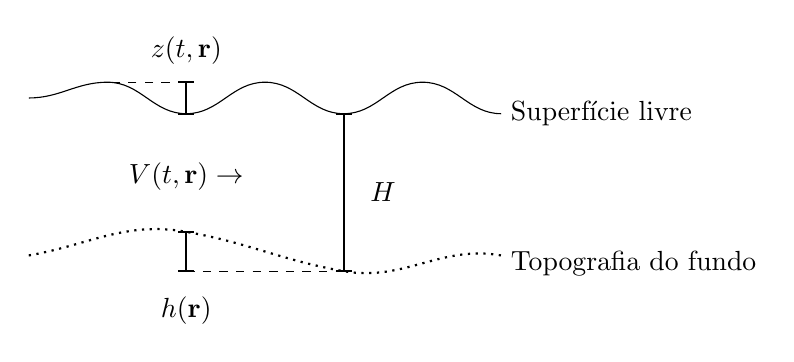
\begin{tikzpicture}[scale=1] 
				
		% Superfície livre
		\draw[above] (0,4) to[out=0,in=180] (1,4.2) 
		to[out=0,in=180] (2,3.8)
		to[out=0,in=180] (3,4.2)
		to[out=0,in=180] (4,3.8)
		to[out=0,in=180] (5,4.2)
		to[out=0,in=180] (6,3.8);
		\node[right] at (6,3.8) {Superfície livre};
				
		% Linha tracejada de referência para z
		\draw[dashed] (2,4.2) -- (1,4.2);
				
		% Desvio da superfície z
		\draw[thick] (2,3.8) -- (2,4.2);
		\draw[thick] (1.9,3.8) -- (2.1,3.8); % traço inferior
		\draw[thick] (1.9,4.2) -- (2.1,4.2); % traço superior
		\node[above] at (2,4.3) {$z(t,\mathbf{r})$};
				
		% Velocidade V(t,r)
		\node at (2,3) {$ V(t,\mathbf{r}) \rightarrow$};
				
		% Profundidade média H
		\draw[thick] (4,3.8) -- (4,1.8);
		\draw[thick] (3.9,3.8) -- (4.1,3.8); % traço superior
		\draw[thick] (3.9,1.8) -- (4.1,1.8); % traço inferior
		\node at (4.5,2.8) {$H$};
				
		% Topografia do fundo (curva inferior)
		\draw[dotted, thick] (0,2) to[out=10,in=170] (2,2.3) 
		to[out=350,in=170] (4,1.8) 
		to[out=350,in=170] (6,2);
		\node[right] at (6,1.9) {Topografia do fundo};
				
		% Variação da topografia h
		\draw[thick] (2,2.3) -- (2,1.8);
		\draw[thick] (1.9,2.3) -- (2.1,2.3); % traço superior
		\draw[thick] (1.9,1.8) -- (2.1,1.8); % traço inferior
		\node[below] at (2,1.6) {$h(\mathbf{r})$};
				
		% Linha tracejada de referência para h
		\draw[dashed] (2,1.8) -- (4,1.8);
				
	\end{tikzpicture}
	\caption{Diagrama do modelo de água-rasa adaptado}
	\label{fig:fluido-topografia}
\end{figure}

Além disso, o modelo de água-rasa adaptado é expresso por:
\begin{align}
	\frac{\partial V}{\partial t} & = - ( V \cdot \nabla)V - f \mathbf{k} \times V - g \nabla z + \nu \nabla^2 V \label{eq:agua-rasa-modificada-1}     \\
	\frac{\partial z}{\partial t} & = - (V \cdot \nabla)(z - h) - (H + z - h)\nabla \cdot  V + \kappa \nabla^2 z + F \label{eq:agua-rasa-modificada-2} 
\end{align}

Onde:
    \begin{itemize}
    	\item $H$: profundidade média do fluido;
    	\item $h(\mathbf{r})$: variação da superfície topológica;
    	\item $V(t,\mathbf{r})$: Velocidade horizontal;
    	\item $z(t,\mathbf{r})$: altura da superfície;
    	\item $F$: forças externas;
    	\item $\kappa$: coeficiente de difusão viscosa;
    	\item $\nu$: coeficiente de difusão térmica;
    \end{itemize}

Em seguida, aplicamos a \textit{decomposição de Helmholtz} à equação \eqref{eq:agua-rasa-modificada-1}, escrevendo
\begin{equation*}
	V = \nabla \chi + \mathbf{k} \times \nabla \psi,
\end{equation*}
onde $\chi$ é o potencial de velocidade associado à parte divergente e $\psi$ a função corrente associada à parte rotacional. Dessa forma, $\nabla^2 \chi$ representa a divergência e $\nabla^2 \psi$ a vorticidade. Substituindo essa decomposição obtemos:
\begin{align}
	\frac{\partial \nabla^2 \chi}{\partial t} & = -\tfrac{1}{2}\nabla^2(\nabla \chi \cdot \nabla \chi) 
	- \nabla \chi \cdot \nabla(\nabla^2\psi) \times \mathbf{k} 
	+ \nabla^2(\nabla \chi \cdot \nabla \psi \times \mathbf{k}) \nonumber \\
    & \quad + \nabla \cdot (\nabla^2\psi\nabla\psi)          
	- \tfrac{1}{2}\nabla^2(\nabla \psi \cdot \nabla \psi) 
	+ \nu\nabla^4\chi + f\nabla^2\psi - g\nabla^2z, \label{eq:equacao-basica-1} \\
	\frac{\partial \nabla^2 \psi}{\partial t} & = -\nabla \cdot (\nabla^2\psi\nabla \chi)              
	- \nabla \psi \cdot \nabla(\nabla^2\psi) \times \mathbf{k} 
	- f\nabla^2\chi + \nu\nabla^4\psi. \label{eq:equacao-basica-2}
\end{align}

Analogamente, aplicando \eqref{eq:agua-rasa-modificada-2}, temos:
\begin{equation}
	\frac{\partial z}{\partial t} 
	= -\nabla \cdot \big[(z - h)\nabla \chi\big] 
	- \nabla \psi \cdot \nabla(z - h) \times \mathbf{k} 
	- H\nabla^2\chi + \kappa\nabla^2z + F. 
	\label{eq:equacao-basica-3}
\end{equation}

Nosso objetivo é reduzir as equações \eqref{eq:equacao-basica-1}–\eqref{eq:equacao-basica-3} a um modelo de baixa ordem. Para isso, introduzimos três vetores adimensionais $\alpha_1, \alpha_2, \alpha_3$ que satisfazem
\begin{equation*}
	\alpha_1 + \alpha_2 + \alpha_3 = 0,
\end{equation*}
e adotamos as permutações cíclicas
\begin{equation*}
	(i,j,k) = (1,2,3),\; (2,3,1),\; (3,1,2).
\end{equation*}
Definimos então:
\begin{equation*}
	a_i = \alpha_i \cdot \alpha_i, 
	\quad b_i = \alpha_j \cdot \alpha_k, 
	\quad c = (b_1b_2+b_2b_3+b_3b_1)^{1/2}.
\end{equation*}

Lorenz também apresenta uma forma alternativa, equivalente, mais conveniente para a implementação computacional:
\begin{equation*}
	b_i = \tfrac{1}{2}(a_i - a_j - a_k), 
	\quad c_i = c.
\end{equation*}

Escolhido um comprimento característico $L$, construímos três funções ortogonais:
\begin{equation*}
	\phi_i(\mathbf{r}) = \cos\!\left(\alpha_i \cdot \frac{\mathbf{r}}{L}\right),
\end{equation*}
para as quais valem, por exemplo:
\begin{align*}
	L^2\nabla^2\phi_i                              & = -a_i\phi_i,                         \\
	L^2\nabla\phi_i \cdot \nabla\phi_k             & = -\tfrac{1}{2}b_{ik}\phi_i + \cdots, \\
	L^2\nabla \cdot (\phi_j\nabla\phi_k)           & = \tfrac{1}{2}b_{jk}\phi_i + \cdots,  \\
	L^2\phi_j \cdot \nabla\phi_k \times \mathbf{k} & = -\tfrac{1}{2}c_{jk}\phi_i + \cdots, 
\end{align*}
onde os termos omitidos são múltiplos de cossenos. Com essas funções, expandimos as variáveis em série e introduzimos escalas adimensionais:
\begin{align*}
	t    & = f^{-1}\tau,               \\
	\chi & = 2L^2f^2 \sum_i x_i\phi_i,                                              \\
	\psi & = 2L^2f^2 \sum_i y_i\phi_i,                                              \\
	z    & = 2L^2f^2g^{-1} \sum_i z_i\phi_i,                                        \\
	h    & = 2L^2f^2g^{-1} \sum_i h_i\phi_i,                                        \\
	F    & = 2L^2f^2g^{-1} \sum_i F_i\phi_i.
\end{align*}

Substituindo as equações acima em \eqref{eq:equacao-basica-1}–\eqref{eq:equacao-basica-3}, e projetando sobre a base $\{\phi_i\}$, obtemos finalmente o modelo PE de baixa ordem, composto de nove equações diferenciais ordinárias:
\begin{align}
    a_i\frac{dx_i}{d\tau} & = a_ib_ix_ix_k - c(a_i - a_k)x_iy_k      
	+ c(a_i - a_j)y_ix_k -2c^2y_iy_k - \nu_0a_i^2x_i + a_iy_i - a_iz_i, \label{eq:modelo-pe-1}\\
	a_i\frac{dy_i}{d\tau} & = -a_ib_kx_iy_k - a_ib_iy_ix_k           
	+ c(a_k - a_i)y_iy_k - a_ix_i - \nu_0a_i^2y_i, \label{eq:modelo-pe-2}\\
	\frac{dz_i}{d\tau}    & = -b_kx_i(z_k - h_k) - b_i(z_i - h_i)x_k 
	+ c\,y_i(z_k - h_k) - c(z_i - h_i)y_k + g_0a_ix_i - \kappa_0a_iz_i + F_i. \label{eq:modelo-pe-3}
\end{align}

onde,
\begin{itemize}
	\item $x_i$ representam os modos divergentes do escoamento (associados às ondas de gravidade);
	\item $y_i$ representam os modos rotacionais (vorticidade), associados às oscilações quasi-geostróficas;
	\item $z_i$ são variáveis auxiliares acopladas ao sistema;
\end{itemize}
Na construção do modelo QG, começamos desprezando todos os termos não lineares, assim como aqueles que envolvem as variáveis $x$, incluindo a derivada temporal, na equação \eqref{eq:modelo-pe-1}. Fazemos o mesmo com os termos não lineares ou topográficos que dependem de $x$ nas equações \eqref{eq:modelo-pe-2} e \eqref{eq:modelo-pe-3}. Por fim, eliminamos as variáveis $x$ e $z$, obtendo ao modelo QG apresentado a seguir:
\begin{equation}
	(a_i g_0 + 1)\,\frac{dy_i}{d\tau} 
	= g_0 c (a_k - a_j) y_j y_k 
	- a_i (a_i g_0 \nu_0 + \kappa_0) y_i 
	- c h_k y_j + c h_j y_k + F_i,
	\label{eq:modelo_lorenz_deterministico_qg}
\end{equation}

\textbf{ADICIONAR SOBRE O CAPÍTULO 2.7 DO SALMON}

\section{Simulações} \label{sec:ch01_simulacoes_deterministico}
Nesta seção, apresentaremos o resultados das simulações computacionais do modelo PE, expresso pelas equações \eqref{eq:modelo-pe-1}-\eqref{eq:modelo-pe-3}. Os gráficos foram gerados a partir de simulações computacionais realizadas em Julia, principalmente, com o auxílio da biblioteca \textit{SciML: Differentiable Modeling and Simulation Combined with Machine Learning} \citep{Rackauckas2017}. 

Os parâmetros usados para a simulação foram os mesmos utilizados em \citet{Lorenz1980} e \cite{Chekroun2021}. Os parâmetros estão definidos a seguir: $g_0 = \SI{8}{\meter\per\square\second}$, $a = (1, 1, 3)$, $F = (0.1, 0, 0)$ e $c = \sqrt{\tfrac{3}{4}}$, $h=(-1, 0, 0)$ e $\nu_0 = \kappa_0 = \frac{1}{48}$. As simulações foram realizadas a partir do código disponível no apêndice \ref{app:apendice-lista-de-programas}.  

\begin{figure}[H]
  \centering
  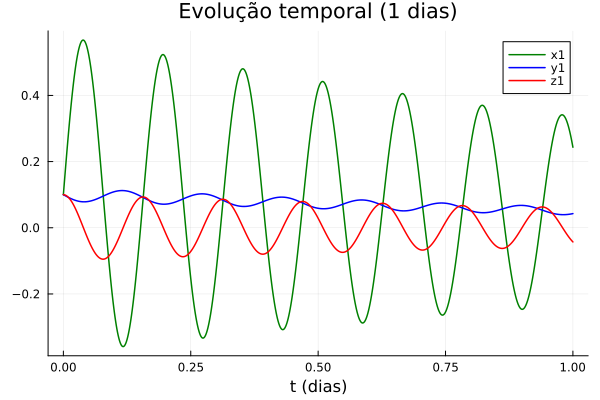
\includegraphics[width=0.6\textwidth]{00_TCC/01_LATEX/figuras/ch01_lorenz_80/evolucao_temporal_01.png}
  \caption{Simulação do modelo PE (1 dia).\label{fig:lorenz80_pe_1}}
\end{figure}

Os parâmetros usados para a simulação foram os mesmos utilizados em \citet{Lorenz1980} e \cite{Chekroun2021}. Os parâmetros estão definidos a seguir: $g_0 = \SI{8}{\meter\per\square\second}$, $a = (1, 1, 3)$, $F = (0.1, 0, 0)$ e $c = \sqrt{\tfrac{3}{4}}$, $h=(-1, 0, 0)$ e $\nu_0 = \kappa_0 = \frac{1}{48}$. As simulações foram realizadas a partir do código disponível no apêndice \ref{app:apendice-lista-de-programas}.  

Os parâmetros usados para a simulação foram os mesmos utilizados em \citet{Lorenz1980} e \cite{Chekroun2021}. Os parâmetros estão definidos a seguir: $g_0 = \SI{8}{\meter\per\square\second}$, $a = (1, 1, 3)$, $F = (0.1, 0, 0)$ e $c = \sqrt{\tfrac{3}{4}}$, $h=(-1, 0, 0)$ e $\nu_0 = \kappa_0 = \frac{1}{48}$. As simulações foram realizadas a partir do código disponível no apêndice \ref{app:apendice-lista-de-programas}.  


\begin{figure}[H]
  \centering
    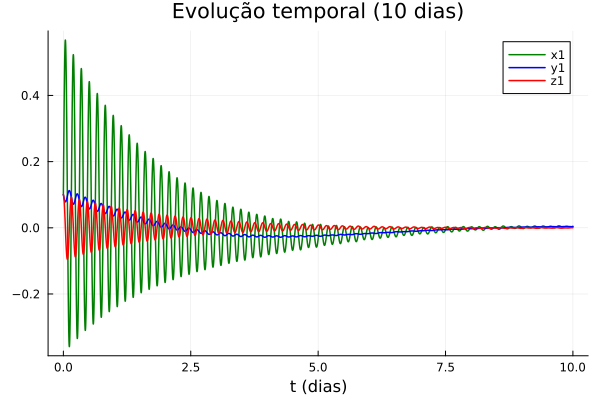
\includegraphics[width=0.75\textwidth]{00_TCC/01_LATEX/figuras/ch01_lorenz_80/evolucao_temporal_10.png}
  \caption{Simulação do modelo PE (10 dias)\label{fig:lorenz80_pe_2}}
\end{figure}

